\documentclass{standalone}
\usepackage{tikz}
\usetikzlibrary{patterns, positioning}


\begin{document}
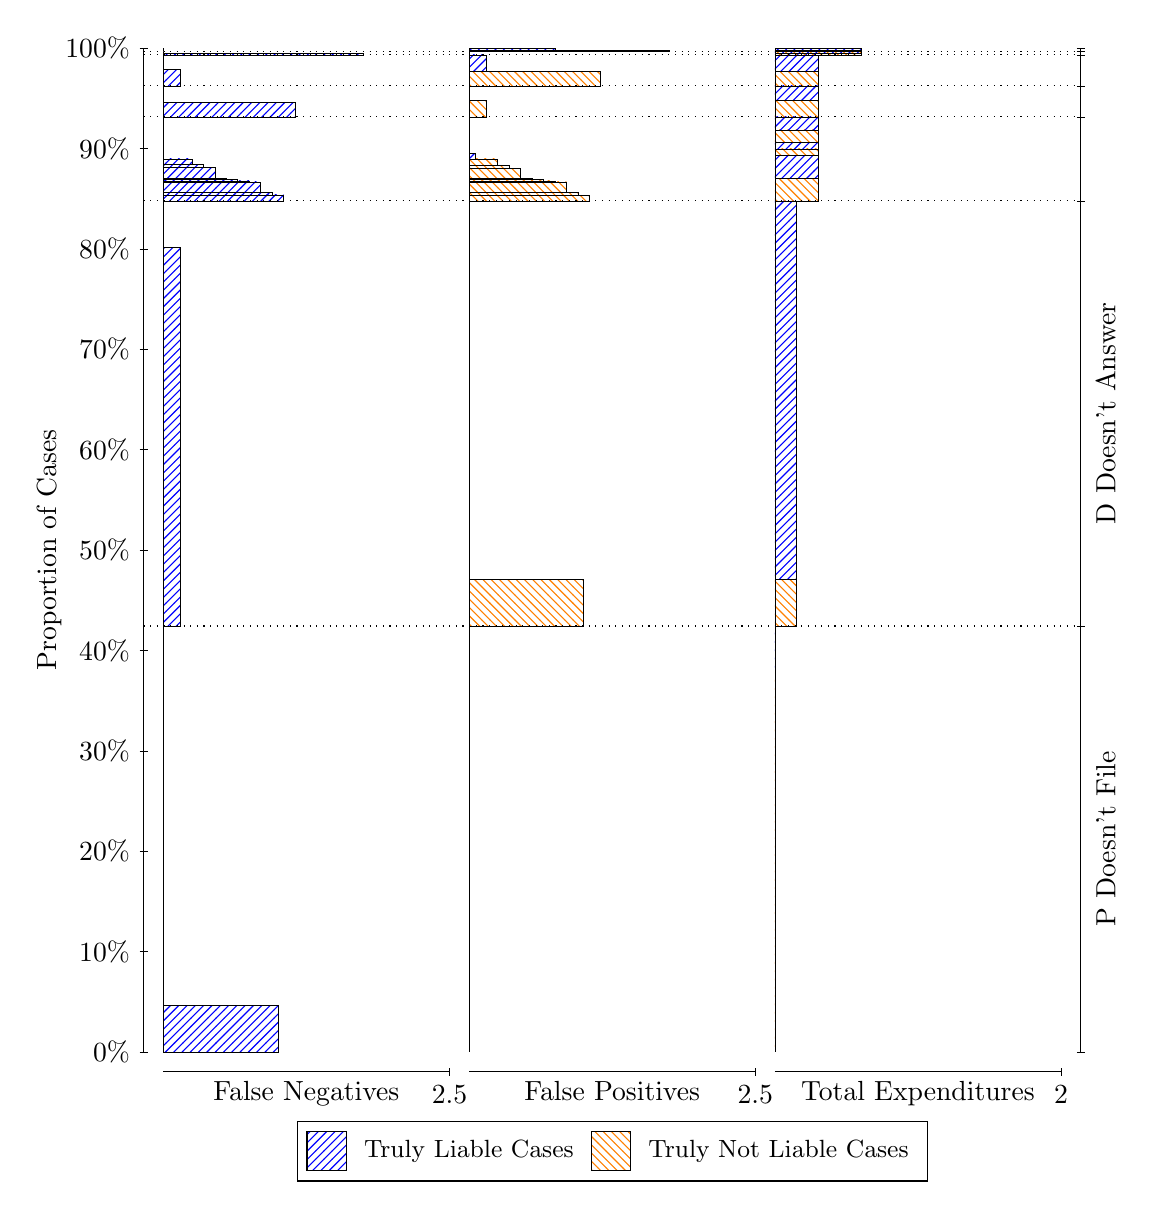
\begin{tikzpicture}
\draw[black, very thin] (1.5,1.75) -- (1.5,14.5);
\node[rotate=90, text=black, anchor=center] at (0.3, 8.125) {Proportion of Cases};
\draw[black, very thin] (1.45,1.75) -- (1.55,1.75);
\node[text=black, anchor=east] at (1.45, 1.75) {0\%};
\draw[black, very thin] (1.45,3.025) -- (1.55,3.025);
\node[text=black, anchor=east] at (1.45, 3.025) {10\%};
\draw[black, very thin] (1.45,4.3) -- (1.55,4.3);
\node[text=black, anchor=east] at (1.45, 4.3) {20\%};
\draw[black, very thin] (1.45,5.575) -- (1.55,5.575);
\node[text=black, anchor=east] at (1.45, 5.575) {30\%};
\draw[black, very thin] (1.45,6.85) -- (1.55,6.85);
\node[text=black, anchor=east] at (1.45, 6.85) {40\%};
\draw[black, very thin] (1.45,8.125) -- (1.55,8.125);
\node[text=black, anchor=east] at (1.45, 8.125) {50\%};
\draw[black, very thin] (1.45,9.4) -- (1.55,9.4);
\node[text=black, anchor=east] at (1.45, 9.4) {60\%};
\draw[black, very thin] (1.45,10.675) -- (1.55,10.675);
\node[text=black, anchor=east] at (1.45, 10.675) {70\%};
\draw[black, very thin] (1.45,11.95) -- (1.55,11.95);
\node[text=black, anchor=east] at (1.45, 11.95) {80\%};
\draw[black, very thin] (1.45,13.225) -- (1.55,13.225);
\node[text=black, anchor=east] at (1.45, 13.225) {90\%};
\draw[black, very thin] (1.45,14.5) -- (1.55,14.5);
\node[text=black, anchor=east] at (1.45, 14.5) {100\%};

\draw[black, very thin] (13.4,1.75) -- (13.4,14.5);
\draw[black, very thin] (13.35,1.75) -- (13.45,1.75);
\node[anchor=west] at (13.35, 1.75) {};
\draw[black, very thin] (13.35,7.1599) -- (13.45,7.1599);
\node[anchor=west] at (13.35, 7.1599) {};
\draw[black, very thin] (13.35,12.559) -- (13.45,12.559);
\node[anchor=west] at (13.35, 12.559) {};
\draw[black, very thin] (13.35,13.625) -- (13.45,13.625);
\node[anchor=west] at (13.35, 13.625) {};
\draw[black, very thin] (13.35,14.02) -- (13.45,14.02);
\node[anchor=west] at (13.35, 14.02) {};
\draw[black, very thin] (13.35,14.413) -- (13.45,14.413);
\node[anchor=west] at (13.35, 14.413) {};
\draw[black, very thin] (13.35,14.457) -- (13.45,14.457);
\node[anchor=west] at (13.35, 14.457) {};
\draw[black, very thin] (13.35,14.5) -- (13.45,14.5);
\node[anchor=west] at (13.35, 14.5) {};

\draw[black, very thin, pattern color=blue, pattern=north east lines] (1.75,1.75) rectangle (3.2033,2.3454);
\draw[black, very thin, pattern color=orange, pattern=north west lines] (1.75,2.3454) rectangle (1.75,7.1599);
\draw[black, very thin, pattern color=blue, pattern=north east lines] (1.75,7.1599) rectangle (1.968,11.969);
\draw[black, very thin, pattern color=orange, pattern=north west lines] (1.75,11.969) rectangle (1.75,12.559);
\draw[black, very thin, pattern color=blue, pattern=north east lines] (1.75,12.559) rectangle (3.276,12.636);
\draw[black, very thin, pattern color=blue, pattern=north east lines] (1.75,12.636) rectangle (3.1307,12.671);
\draw[black, very thin, pattern color=blue, pattern=north east lines] (1.75,12.671) rectangle (2.9853,12.799);
\draw[black, very thin, pattern color=blue, pattern=north east lines] (1.75,12.799) rectangle (2.84,12.812);
\draw[black, very thin, pattern color=blue, pattern=north east lines] (1.75,12.812) rectangle (2.6947,12.834);
\draw[black, very thin, pattern color=blue, pattern=north east lines] (1.75,12.834) rectangle (2.5493,12.847);
\draw[black, very thin, pattern color=blue, pattern=north east lines] (1.75,12.847) rectangle (2.404,12.982);
\draw[black, very thin, pattern color=blue, pattern=north east lines] (1.75,12.982) rectangle (2.2587,13.018);
\draw[black, very thin, pattern color=blue, pattern=north east lines] (1.75,13.018) rectangle (2.1133,13.092);
\draw[black, very thin, pattern color=orange, pattern=north west lines] (1.75,13.092) rectangle (1.75,13.625);
\draw[black, very thin, pattern color=blue, pattern=north east lines] (1.75,13.625) rectangle (3.4213,13.811);
\draw[black, very thin, pattern color=orange, pattern=north west lines] (1.75,13.811) rectangle (1.75,14.02);
\draw[black, very thin, pattern color=blue, pattern=north east lines] (1.75,14.02) rectangle (1.968,14.227);
\draw[black, very thin, pattern color=orange, pattern=north west lines] (1.75,14.227) rectangle (1.75,14.413);
\draw[black, very thin, pattern color=blue, pattern=north east lines] (1.75,14.413) rectangle (4.2933,14.431);
\draw[black, very thin, pattern color=orange, pattern=north west lines] (1.75,14.431) rectangle (1.75,14.457);
\draw[black, very thin, pattern color=orange, pattern=north west lines] (1.75,14.457) rectangle (1.75,14.474);
\draw[black, very thin, pattern color=blue, pattern=north east lines] (1.75,14.474) rectangle (1.75,14.5);
\draw[black, very thin, pattern color=orange, pattern=north west lines] (5.6333,1.75) rectangle (5.6333,6.5646);
\draw[black, very thin, pattern color=blue, pattern=north east lines] (5.6333,6.5646) rectangle (5.6333,7.1599);
\draw[black, very thin, pattern color=orange, pattern=north west lines] (5.6333,7.1599) rectangle (7.0867,7.7497);
\draw[black, very thin, pattern color=blue, pattern=north east lines] (5.6333,7.7497) rectangle (5.6333,12.559);
\draw[black, very thin, pattern color=orange, pattern=north west lines] (5.6333,12.559) rectangle (7.1593,12.628);
\draw[black, very thin, pattern color=orange, pattern=north west lines] (5.6333,12.628) rectangle (7.014,12.664);
\draw[black, very thin, pattern color=orange, pattern=north west lines] (5.6333,12.664) rectangle (6.8687,12.799);
\draw[black, very thin, pattern color=orange, pattern=north west lines] (5.6333,12.799) rectangle (6.7233,12.812);
\draw[black, very thin, pattern color=orange, pattern=north west lines] (5.6333,12.812) rectangle (6.578,12.834);
\draw[black, very thin, pattern color=orange, pattern=north west lines] (5.6333,12.834) rectangle (6.4327,12.847);
\draw[black, very thin, pattern color=orange, pattern=north west lines] (5.6333,12.847) rectangle (6.2873,12.975);
\draw[black, very thin, pattern color=orange, pattern=north west lines] (5.6333,12.975) rectangle (6.142,13.01);
\draw[black, very thin, pattern color=orange, pattern=north west lines] (5.6333,13.01) rectangle (5.9967,13.092);
\draw[black, very thin, pattern color=blue, pattern=north east lines] (5.6333,13.092) rectangle (5.706,13.166);
\draw[black, very thin, pattern color=blue, pattern=north east lines] (5.6333,13.166) rectangle (5.6333,13.625);
\draw[black, very thin, pattern color=orange, pattern=north west lines] (5.6333,13.625) rectangle (5.8513,13.833);
\draw[black, very thin, pattern color=blue, pattern=north east lines] (5.6333,13.833) rectangle (5.6333,14.02);
\draw[black, very thin, pattern color=orange, pattern=north west lines] (5.6333,14.02) rectangle (7.3047,14.206);
\draw[black, very thin, pattern color=blue, pattern=north east lines] (5.6333,14.206) rectangle (5.8513,14.413);
\draw[black, very thin, pattern color=orange, pattern=north west lines] (5.6333,14.413) rectangle (5.6333,14.439);
\draw[black, very thin, pattern color=blue, pattern=north east lines] (5.6333,14.439) rectangle (5.6333,14.457);
\draw[black, very thin, pattern color=orange, pattern=north west lines] (5.6333,14.457) rectangle (8.1767,14.474);
\draw[black, very thin, pattern color=blue, pattern=north east lines] (5.6333,14.474) rectangle (6.7233,14.5);
\draw[black, very thin, pattern color=orange, pattern=north west lines] (9.5167,1.75) rectangle (9.5167,6.5646);
\draw[black, very thin, pattern color=blue, pattern=north east lines] (9.5167,6.5646) rectangle (9.5167,7.1599);
\draw[black, very thin, pattern color=orange, pattern=north west lines] (9.5167,7.1599) rectangle (9.7892,7.7497);
\draw[black, very thin, pattern color=blue, pattern=north east lines] (9.5167,7.7497) rectangle (9.7892,12.559);
\draw[black, very thin, pattern color=orange, pattern=north west lines] (9.5167,12.559) rectangle (10.062,12.847);
\draw[black, very thin, pattern color=blue, pattern=north east lines] (9.5167,12.847) rectangle (10.062,13.139);
\draw[black, very thin, pattern color=orange, pattern=north west lines] (9.5167,13.139) rectangle (10.062,13.22);
\draw[black, very thin, pattern color=blue, pattern=north east lines] (9.5167,13.22) rectangle (10.062,13.297);
\draw[black, very thin, pattern color=orange, pattern=north west lines] (9.5167,13.297) rectangle (10.062,13.461);
\draw[black, very thin, pattern color=blue, pattern=north east lines] (9.5167,13.461) rectangle (10.062,13.625);
\draw[black, very thin, pattern color=orange, pattern=north west lines] (9.5167,13.625) rectangle (10.062,13.833);
\draw[black, very thin, pattern color=blue, pattern=north east lines] (9.5167,13.833) rectangle (10.062,14.02);
\draw[black, very thin, pattern color=orange, pattern=north west lines] (9.5167,14.02) rectangle (10.062,14.206);
\draw[black, very thin, pattern color=blue, pattern=north east lines] (9.5167,14.206) rectangle (10.062,14.413);
\draw[black, very thin, pattern color=orange, pattern=north west lines] (9.5167,14.413) rectangle (10.607,14.439);
\draw[black, very thin, pattern color=blue, pattern=north east lines] (9.5167,14.439) rectangle (10.607,14.457);
\draw[black, very thin, pattern color=orange, pattern=north west lines] (9.5167,14.457) rectangle (10.607,14.474);
\draw[black, very thin, pattern color=blue, pattern=north east lines] (9.5167,14.474) rectangle (10.607,14.5);
\draw[black, dotted] (1.5,7.1599) -- (13.4,7.1599);
\draw[black, dotted] (1.5,12.559) -- (13.4,12.559);
\draw[black, dotted] (1.5,13.625) -- (13.4,13.625);
\draw[black, dotted] (1.5,14.02) -- (13.4,14.02);
\draw[black, dotted] (1.5,14.413) -- (13.4,14.413);
\draw[black, dotted] (1.5,14.457) -- (13.4,14.457);
\draw[black, very thin] (1.75,1.5) -- (5.3833,1.5);
\node[text=black, anchor=north] at (3.5667, 1.5) {False Negatives};
\draw[black, very thin] (5.3833,1.45) -- (5.3833,1.55);
\node[text=black, anchor=north] at (5.3833, 1.45) {2.5};

\draw[black, very thin] (5.6333,1.5) -- (9.2667,1.5);
\node[text=black, anchor=north] at (7.45, 1.5) {False Positives};
\draw[black, very thin] (9.2667,1.45) -- (9.2667,1.55);
\node[text=black, anchor=north] at (9.2667, 1.45) {2.5};

\draw[black, very thin] (9.5167,1.5) -- (13.15,1.5);
\node[text=black, anchor=north] at (11.333, 1.5) {Total Expenditures};
\draw[black, very thin] (13.15,1.45) -- (13.15,1.55);
\node[text=black, anchor=north] at (13.15, 1.45) {2};

\node[text=black, centered, rotate=90] at (13.72, 4.455) {P Doesn't File};
\node[text=black, centered, rotate=90] at (13.72, 9.8593) {D Doesn't Answer};






\draw (7.449999999999999,1.5) node[draw=none] (baseCoordinate) {};
\begin{scope}[align=center]
        \matrix[scale=0.5, draw=black, below=0.5cm of baseCoordinate, nodes={draw}, column sep=0.1cm]{
            \node[rectangle, draw, minimum width=0.5cm, minimum height=0.5cm, pattern color=blue, pattern=north east lines] {}; &
            \node[draw=none, font=\small, text=black] (B) {Truly Liable Cases}; &
            \node[rectangle, draw, minimum width=0.5cm, minimum height=0.5cm, pattern color=orange, pattern=north west lines] {}; &
            \node[draw=none, font=\small, text=black] (B) {Truly Not Liable Cases}; \\
            };
\end{scope}

\end{tikzpicture}
\end{document}